% chapter4.tex
% LED Chapter (Muon?)
As described in Chapter \ref{chap:muon}, the four extra modules added in 2010 covering the gap of veto system are equipped with LEDs. M7 and M8 have three LEDs: one at the center and the other two at two ends. M15 and M16 both have one LED installed at the center. The LEDs send out pulses every eight hours. The LED data are used to perform a stability controll of the $\upmu$-veto system. They are clearly defined comparing to muon induced events, therefore the LED events are good probe to estimate the long term stability of these four modules.
\section{Data selection}
The data of muon-veto Run70 to Run138 are used to analyze the aging effect of the veto system. This corresponds to a date from 24.08.2010 to 28.03.2017. When converting the raw data to ROOT-format, the events induced by LED firing are flagged. Therefore, they are easily separated from other events.
The LEDs fire three times every day. Each LED fires 60 pulses in one minute and they fire one after another, which also allows a separation of signals from different LEDs in M7 and M8.



\section{Data Analysis}
The LEDs are fixed on the modules, so the energy spectrum is not smeared by the position dependent light readout. Also, the LEDs are supposed to have constant light output over short time. Thus the obtained ADC spectrum can be fitted with a gaussian function to get the average ADC values of several series.
To increase the statistical power of a single point, events of nine shot series (three days) are combined to perfom a gaussian fit. An example of such fit is illustrated in fig.\ref{fig:gaussian-fit}.

\begin{figure}[htb!]
  \centering
  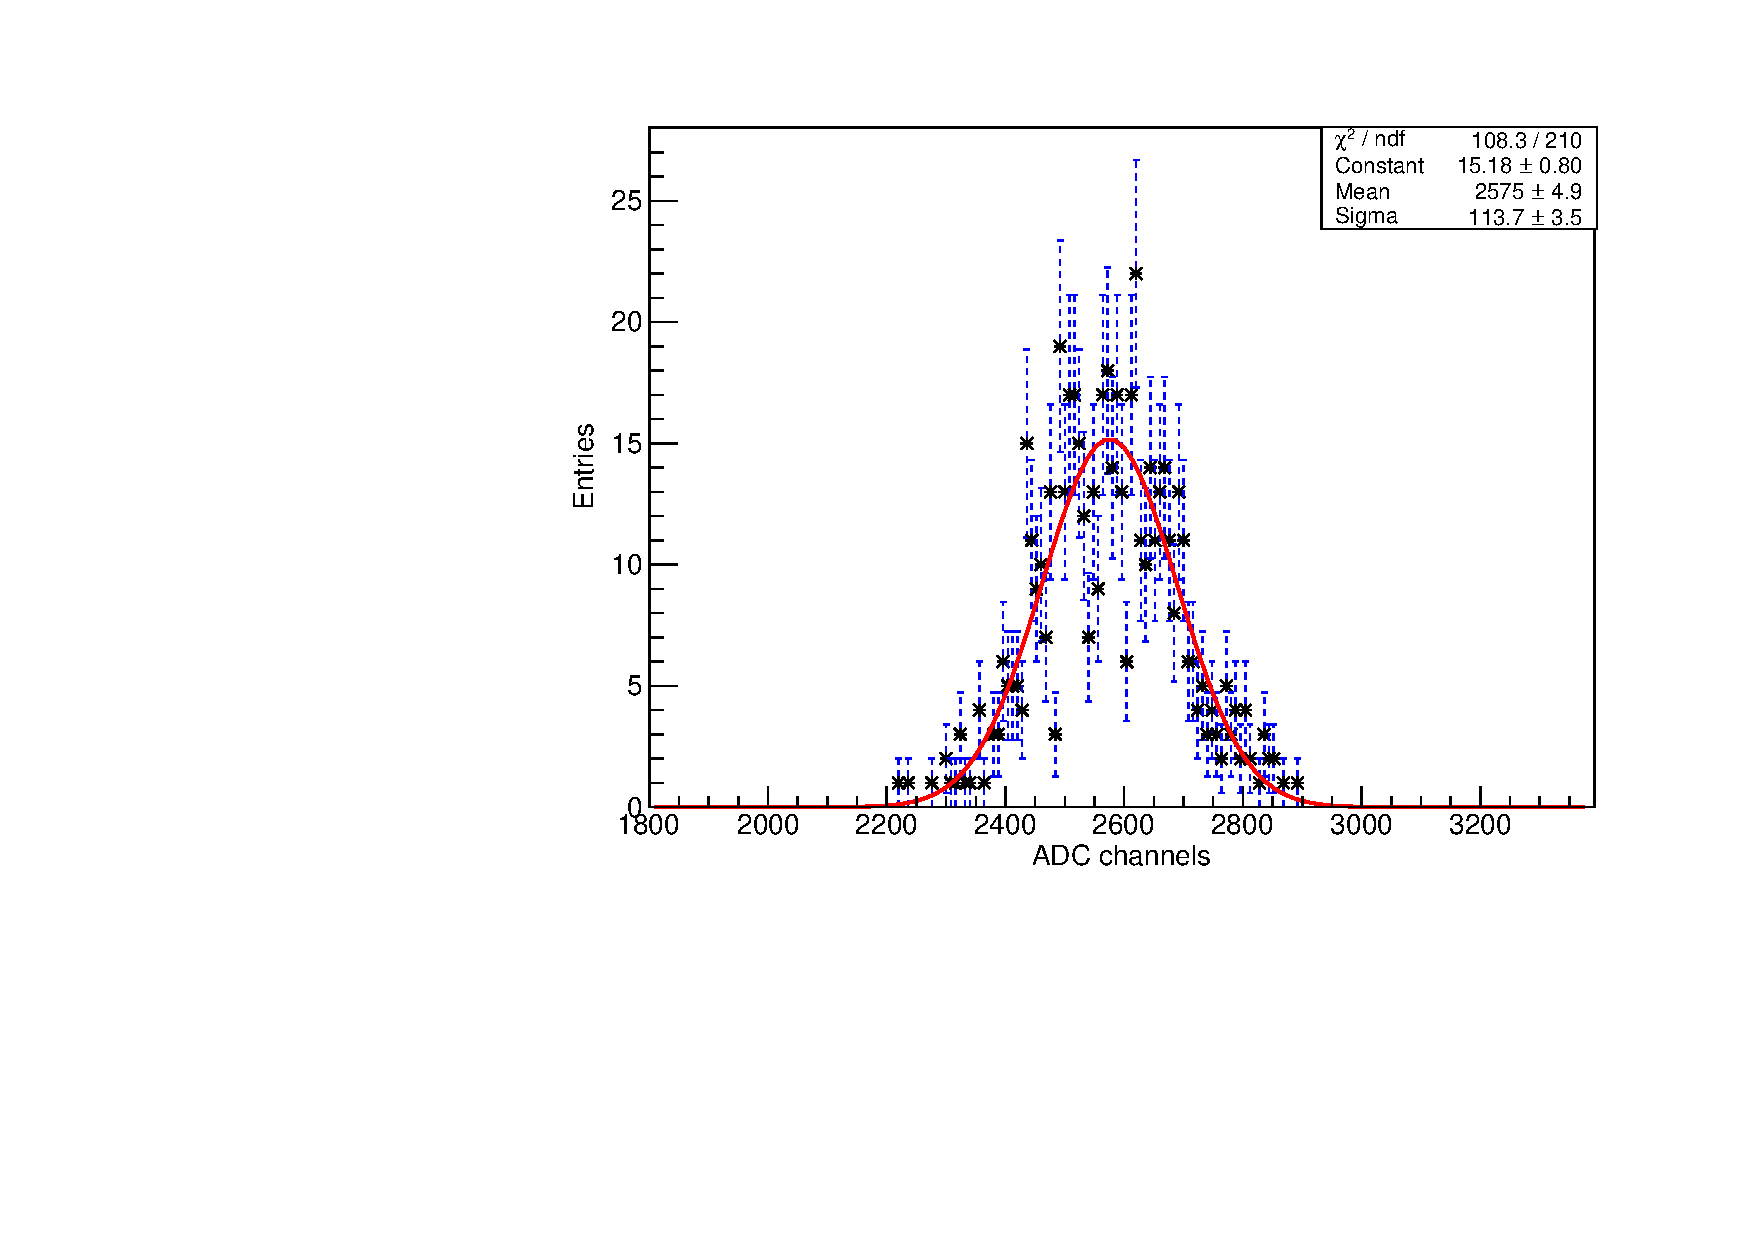
\includegraphics[width=0.5\textwidth{}]{./fig/gaussianM8.pdf}
  \caption{Example of an gaussian fit to nine LED fire series in Module 8, north PMT group. The spectrum is fitted with log likelihood method in ROOT.}
  \label{fig:gaussian-fit}
\end{figure}

The mean ADC values obtained from each gaussian fit are plotted over time. A change of these values over time could be due to various effects, e.g. decrease of the LED light output, aging of scintillator modules, problem of the PMTs or readout elctronics. To identify the contribution of different factors, the values are plotted separately for two PMT groups and three LEDs (for M7 and M8). Linear regressions are made for each data set, see fig.\ref{fig:M8LED}. The lines with different color represent the data from different LEDs. In the following, the result is described in detail for a sample module M8.

\begin{figure}[htbp]
  \centering
  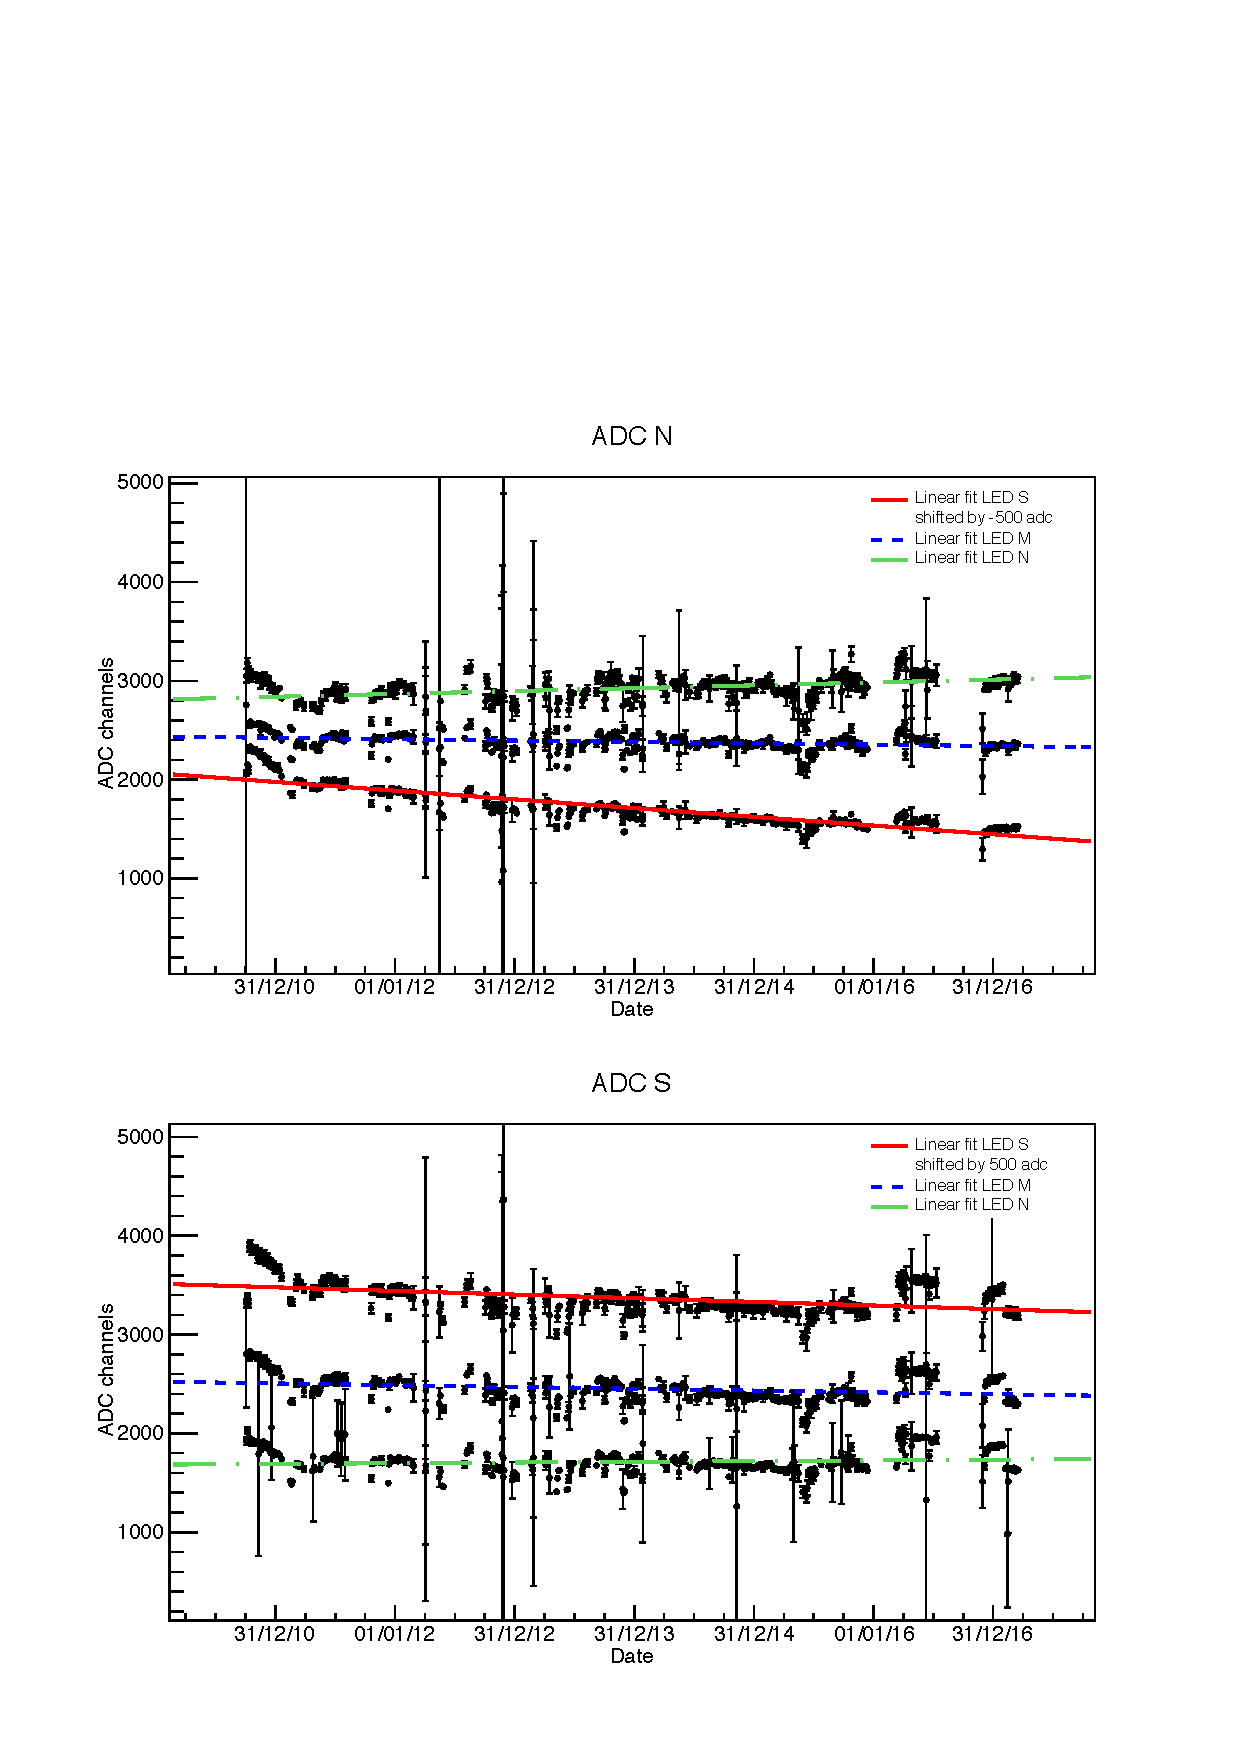
\includegraphics[width=\textwidth{}]{./fig/M8LED.pdf}
  \caption{\textbf{The ADC values of LED signals over time in Module 8.}} The energy deposit of LED signals in ADC channels from Run70 to Run138 are plotted separately for 2 PMT groups (north in upper chart, south in lower chart). The trend of ADC values of different LEDs over time are approximated by linear fits: the green line (LED north), the blue line (LED middle), and the red line (LED south). For clarity reasons, the signals of the south LED are decreased by 500 channels in upper chart and increased by 500 in lower chart.
  \label{fig:M8LED}
\end{figure}

As can be seen in the figure, the mean ADC values of two off-center LEDs differ about 1000 channels from the far end to the near end. Since M7 and M8 are ongly half the length of other top modules, such position dependent effect are even more remarkable in other modules.

\begin{table}[hb]
  \centering
  \caption{Slopes of the linear regressions of 3 LEDs in M8. The first error is statistical error from the linear fit, the second is estimated systematic error. }
  \label{tab:led}
  \begin{tabular}{c c c c}
  \toprule
        & \multicolumn{3}{c}{slope in channels/month} \\
        & LED S   & LED M  & LED N \\
  \midrule
  ADC N & $-7.26\pm0.05\pm4.32$ & $-1.13\pm0.05\pm1.06$ & $2.37\pm0.07\pm3.12$  \\
  ADC S & $-3.02\pm0.07\pm5.50$ & $-1.49\pm0.06\pm2.92$ & $0.59\pm0.05\pm2.74$  \\
  \bottomrule
  \end{tabular}

\end{table}

In fig.\ref{fig:M8LED} , the error bar of a single data point is the statistical error given by the gaussian fit. Since most LED events in one fire serie have good gaussian form, the statistical error is mostly much smaller than the actually error. Several other effects lead to the fluctuation of the ADC value, for example, the switch-on effect of electronics after a long pause. Consequently, the systematic error can only be approximated. The result of the linear fits are listed in Tab.\ref{tab:led} with errors. The systematic error of the slope is estimated by fitting different parts of the time period and taking the difference of the maximum and minimum slopes.

\subsection{Interpretaion of the results}


Various effect could lead to the decrease of mean ADC value of LED events. First, the transparency of plastic scintillator decreases over time. Assuming that such aging effect is homogeneous in one module, the loss of light output depends on the distance from the event position to the PMT group. This leads to roughly the same decrease for events that have same track length to the PMT group, e.g. LED N to ADC S and LED S to ADC N. Second, the PMTs as well as the junction of scintillator module and PMT group have aged individually, which leads to different variation of ADC values at two ends of a module. Last, light output of a LED varies over time and leads to simultaneous change of value measured in two PMT groups.

The slopes of middle LED in two ends of M8 are about the same, implying that the two PMT groups of M8 have aged similarily. Therefore the aging effect of the plastic scintillator can be estimated by subtracting the slope of same LED at far end from the one at near end.
Furthermore the decrease is noticeably more rapid at earlier stage (about 2010-2011) and becomes flat later. The reason can be that the transparency loss of scintillator is not linear over time. The assumption of linear trend is thus only an approximation.
Averaging over time, the decrease due to aging of plastic scintillator is estimated to be $\approx \SI{3}{channels\per month}$.
During the total period of experiment ($\approx\SI{90}{months}$) the change of ADC values is about $\SI{250}{channels}$ for M8.

Same procedure is applied on other three modules M7,M15 and M16 and shows similar results. Since other modules are longer then the four modules, the decrease of ADC values are expected to be more significant. The detection efficiency reduces especially for events to be measured in far PMT group, as the transportaion length of light is longer.
